\documentclass[10.5pt,a4paper]{article}

\usepackage[utf8]{inputenc}
\usepackage[T1]{fontenc}
\usepackage{lmodern}
\usepackage{amsmath,amssymb,amsthm,mathtools,bm}
\usepackage{geometry}
\usepackage{booktabs}
\usepackage{tabularx}
\usepackage{array}
\usepackage{longtable}
\usepackage{graphicx}
\usepackage{xcolor}
\usepackage[hyphens]{url}
\usepackage{hyperref}

\geometry{margin=0.75in}

\definecolor{linkblue}{HTML}{1D4ED8}

\hypersetup{
  colorlinks=true,
  linkcolor=linkblue,
  citecolor=linkblue,
  urlcolor=linkblue,
  pdftitle={Methods and Provenance: Resolving D'Arcy Thompson's 1917 Fish Transformations Paradox and Phylogenetic Prediction Engine},
  pdfauthor={Joel Dietz (Project Delphi)}
}

\Urlmuskip=0mu plus 2mu\relax
\newcommand{\code}[1]{{\footnotesize\nolinkurl{#1}}}

\newcolumntype{L}[1]{>{\raggedright\arraybackslash}p{#1}}
\newcolumntype{Y}{>{\raggedright\arraybackslash}X}

\setlength{\parskip}{0.42em}
\setlength{\parindent}{0pt}
\sloppy

\title{\textbf{Methods \& Provenance: Resolving D'Arcy Thompson's 1917 Fish Transformations Paradox \& Phylogenetic Prediction Engine}}
\author{\textbf{Primary Author:} Joel Dietz (\href{https://github.com/fractastical/morpholib}{Project Delphi})}
\date{October 22, 2026}

\begin{document}
\maketitle

\noindent\textbf{Companion Documents:}
\begin{itemize}
  \setlength{\itemsep}{2pt}
  \item \textbf{Academic Manuscript PDF (31 pages):} \code{docs/thompson_1917_fish_transformations_manuscript.pdf} (\texttt{.tex} source)
  \item \textbf{Visual Guide PDF (11 pages, 13-Year-Old Level):} \code{docs/thompson_1917_visual_guide_for_everyone.pdf} (\code{docs/EXPLAINED_FOR_EVERYONE.md})
  \item \textbf{Registered Predictions \& Fossil Tests:} \code{docs/THOMPSON_PHYLOGENETIC_PREDICTIONS.md}
  \item \textbf{Blind Preregistration \& Scoring vs.\ FishShapes v1:} \code{docs/THOMPSON_BLIND_PREREGISTRATION.md} $\cdot$ \code{docs/THOMPSON_BLIND_TEST_RESULTS.md}
  \item \textbf{Forward Dataset Portfolio \& Unattended Scoring Status:} \code{docs/THOMPSON_DATASET_PORTFOLIO.md} $\cdot$ \code{docs/portfolio/PORTFOLIO_STATUS.md} $\cdot$ \code{docs/portfolio/fishbase_morphmet.md} $\cdot$ \code{docs/portfolio/vespinae_wings.md}
  \item \textbf{Full 43-Turn Discovery \& Peer-Review Chat Log:} \code{docs/THOMPSON_1917_DISCOVERY_CHAT_LOG.md} (\code{docs/thompson_1917_discovery_chat_log.jsonl})
\end{itemize}

\vspace{0.3em}
\hrule
\vspace{0.5em}

\section*{Executive Summary}

This document records the exact computational, statistical, formal-verification, knowledge-graph, and multi-agent methods used to produce the D'Arcy Thompson (1917) fish transformations study, the $10{,}303$-species morphospace-versus-competition synthesis, and the pre-registered blind phylogenetic prediction tests. Specifically, it answers four methodological questions:
\begin{enumerate}
  \setlength{\itemsep}{3pt}
  \item \textbf{What AI / LLM and mathematical models were used} (and what role each played across code generation, blinded multi-provider auditing, remediation, and statistical modeling)?
  \item \textbf{Did we query or publish to the Knowledge Graph (KG)}, and how did the RDF/SPARQL/SQLite and Nanopublication infrastructure drive the research loop?
  \item \textbf{What other code and tooling in this repository were reused or adapted} for the Thompson work?
  \item \textbf{How was scientific rigor enforced} (SHA-256 data pinning, independent pixel re-derivation, machine-checked Lean 4 proofs, domain-expert critique from Prof.\ Peter C.\ Wainwright, and cryptographic pre-registration before unblinding)?
\end{enumerate}

\section{Models Used: Both AI/LLM Agent Models and Mathematical/Evolutionary Models}

Because ``models'' in a computational biology workflow refers both to the \textbf{AI/LLM agent models} used to build and audit the pipeline and to the \textbf{mathematical, morphometric, and phylogenetic models} fitted to the biological data, we document both explicitly.

\subsection{AI / LLM Models \& Blinded Cross-Provider Referee Architecture}

The Thompson investigation was executed inside Cursor using the repository's \textbf{12-Step MorphoEval Closed-Loop Protocol}, which pairs a primary builder/researcher agent with blinded cross-provider referee assessors so no model evaluates its own un-audited assumptions:

\vspace{0.3em}
{\small
\renewcommand{\arraystretch}{1.26}
\begin{tabularx}{\textwidth}{L{1.25in} L{0.82in} L{1.35in} Y}
\toprule
\textbf{Model Identifier} & \textbf{Provider} & \textbf{Role in Investigation} & \textbf{Specific Artifacts \& Contributions} \\
\midrule
\code{claude-fable-5-1} (\code{claude-fable-5-1-thinking-high}) &
Anthropic &
\textbf{Initial Script Builder, Pass 1 \& Pass 2 Primary MorphoEval Assessor, \& Prediction Engine / Blind-Test Architect} &
$\bullet$ Built \code{thompson/1917-thompson-scarus-pomacanthus.py} (\texttt{3cf7f8c4}, \texttt{98520757}).\newline
$\bullet$ Conducted the primary MorphoEval Pass 1 audit (\code{2026-10-16-thompson-audit}, score $70.2/100$) and Pass 2 re-score (\code{2026-10-17-thompson-audit}, score $76.6/100$, \code{morphoeval/audits/2026-10-17-thompson-audit.yaml}).\newline
$\bullet$ Wrote the explicit \textbf{6-item \texttt{remediation} agenda} in \code{2026-10-17-thompson-audit.yaml} (lines 330--337) that directly triggered the 600-point direct outline fitting study.\newline
$\bullet$ Built the linearized 7-mode Phylogenetic Prediction Engine (\code{thompson/run_phylogenetic_prediction_engine.py}), Monte Bolca fossil test, and FishShapes v1 blind preregistration \& scoring pipeline (\code{thompson/preregister_blind_predictions.py}, \code{thompson/score_blind_predictions.py}). \\
\midrule
\code{gemini-4-argon} (\code{gemini-4-argon-medium}) &
Google DeepMind &
\textbf{Blinded Second Assessor (Pass 2) \& Interactive Discovery / Multi-Dataset Synthesis Agent (Turns 1--43)} &
$\bullet$ Executed the blinded second-assessor MorphoEval pass (\code{2026-10-17-blinded-sample-audit}, score $90.8/100$; panel mean $83.7/100$, \code{thompson-scarus-pomacanthus-overall.trig}).\newline
$\bullet$ Conducted the 43-turn interactive research dialogue recorded in \code{docs/THOMPSON_1917_DISCOVERY_CHAT_LOG.md} (transcript \code{0e50eb21-062e-47c3-9ded-1b0bbe630bee}): built the 4-family 791-species atlas (\code{1917-thompson-four-families-atlas.py}), the 600-point silhouette area-paradox solver (\code{1917-thompson-silhouette-area-paradox.py}), the 4 rigor stress-tests (\code{run_rigor_stress_tests.py}), the 600-pt method benchmark \& phylomorphospace analysis (\code{run_wainwright_600pt_and_convergence_tests.py}), the $\bm{G}$ vs.\ $\bm{R}$ competition decomposition (\code{run_morphospace_vs_competition_analysis.py}), the 3-dataset $10{,}303$-species replication (\code{run_three_dataset_validation.py}), the 4-parameter Box-vs.-Warping deconfounding audit (\code{run_box_vs_warping_audit.py}), and the 4 PCM downstream implications (\code{run_pcm_downstream_implications.py}). \\
\midrule
\textbf{Human PI \& Domain-Expert Feedback} &
Joel Dietz (PI) \& Prof.\ Peter C.\ Wainwright (UC Davis) &
\textbf{Hypothesis Challenging, Visual Skepticism, \& Methodological Benchmarking} &
$\bullet$ \textbf{Joel Dietz (Turns 2, 9, 24--25, 33, 35, 37):} Challenged the 17-landmark polygon stick figures (\emph{``I have a hard time seeing that the simplifications of the fish forms lead to the result you are saying''}, Turn 9), which forced the direct 600-point silhouette overlay and uncovered the \textbf{9/17 head-landmark seesaw paradox}; demanded external dataset validation beyond 791 species (Turn 35 $\to 6{,}614$ and $10{,}303$ species); and asked whether the 600-point fit was merely doing a trivial box stretch rather than Thompson's actual skew/curvature claims (Turn 37 $\to$ \code{run_box_vs_warping_audit.py}).\newline
$\bullet$ \textbf{Prof.\ Peter C.\ Wainwright (UC Davis, Turns 22--28):} Co-creator of the 791-species reef-fish dataset; his email feedback on Panel E (\texttt{\% Reaching Genus Noise Floor}), standard 600-semilandmark outline methods (EFD / curve TPS), and convergent evolution directly motivated Sections 1.5--1.6 and \code{run_wainwright_600pt_and_convergence_tests.py}. \\
\bottomrule
\end{tabularx}
}

\subsection{System Architecture, Closed-Loop Integration \& Component-to-Component Data Contracts}

To eliminate ambiguity about how frontier LLM agents, human investigators, deterministic Python/Lean 4 verifiers, and the Project Delphi RDF Knowledge Graph interact, the figure below (generated deterministically by \code{thompson/generate_architecture_diagram.py} $\to$ \code{docs/thompson_system_architecture_and_dataflow.png}) depicts the \textbf{three coupled closed loops} and the exact file/schema payloads passed across every edge.

\begin{center}
  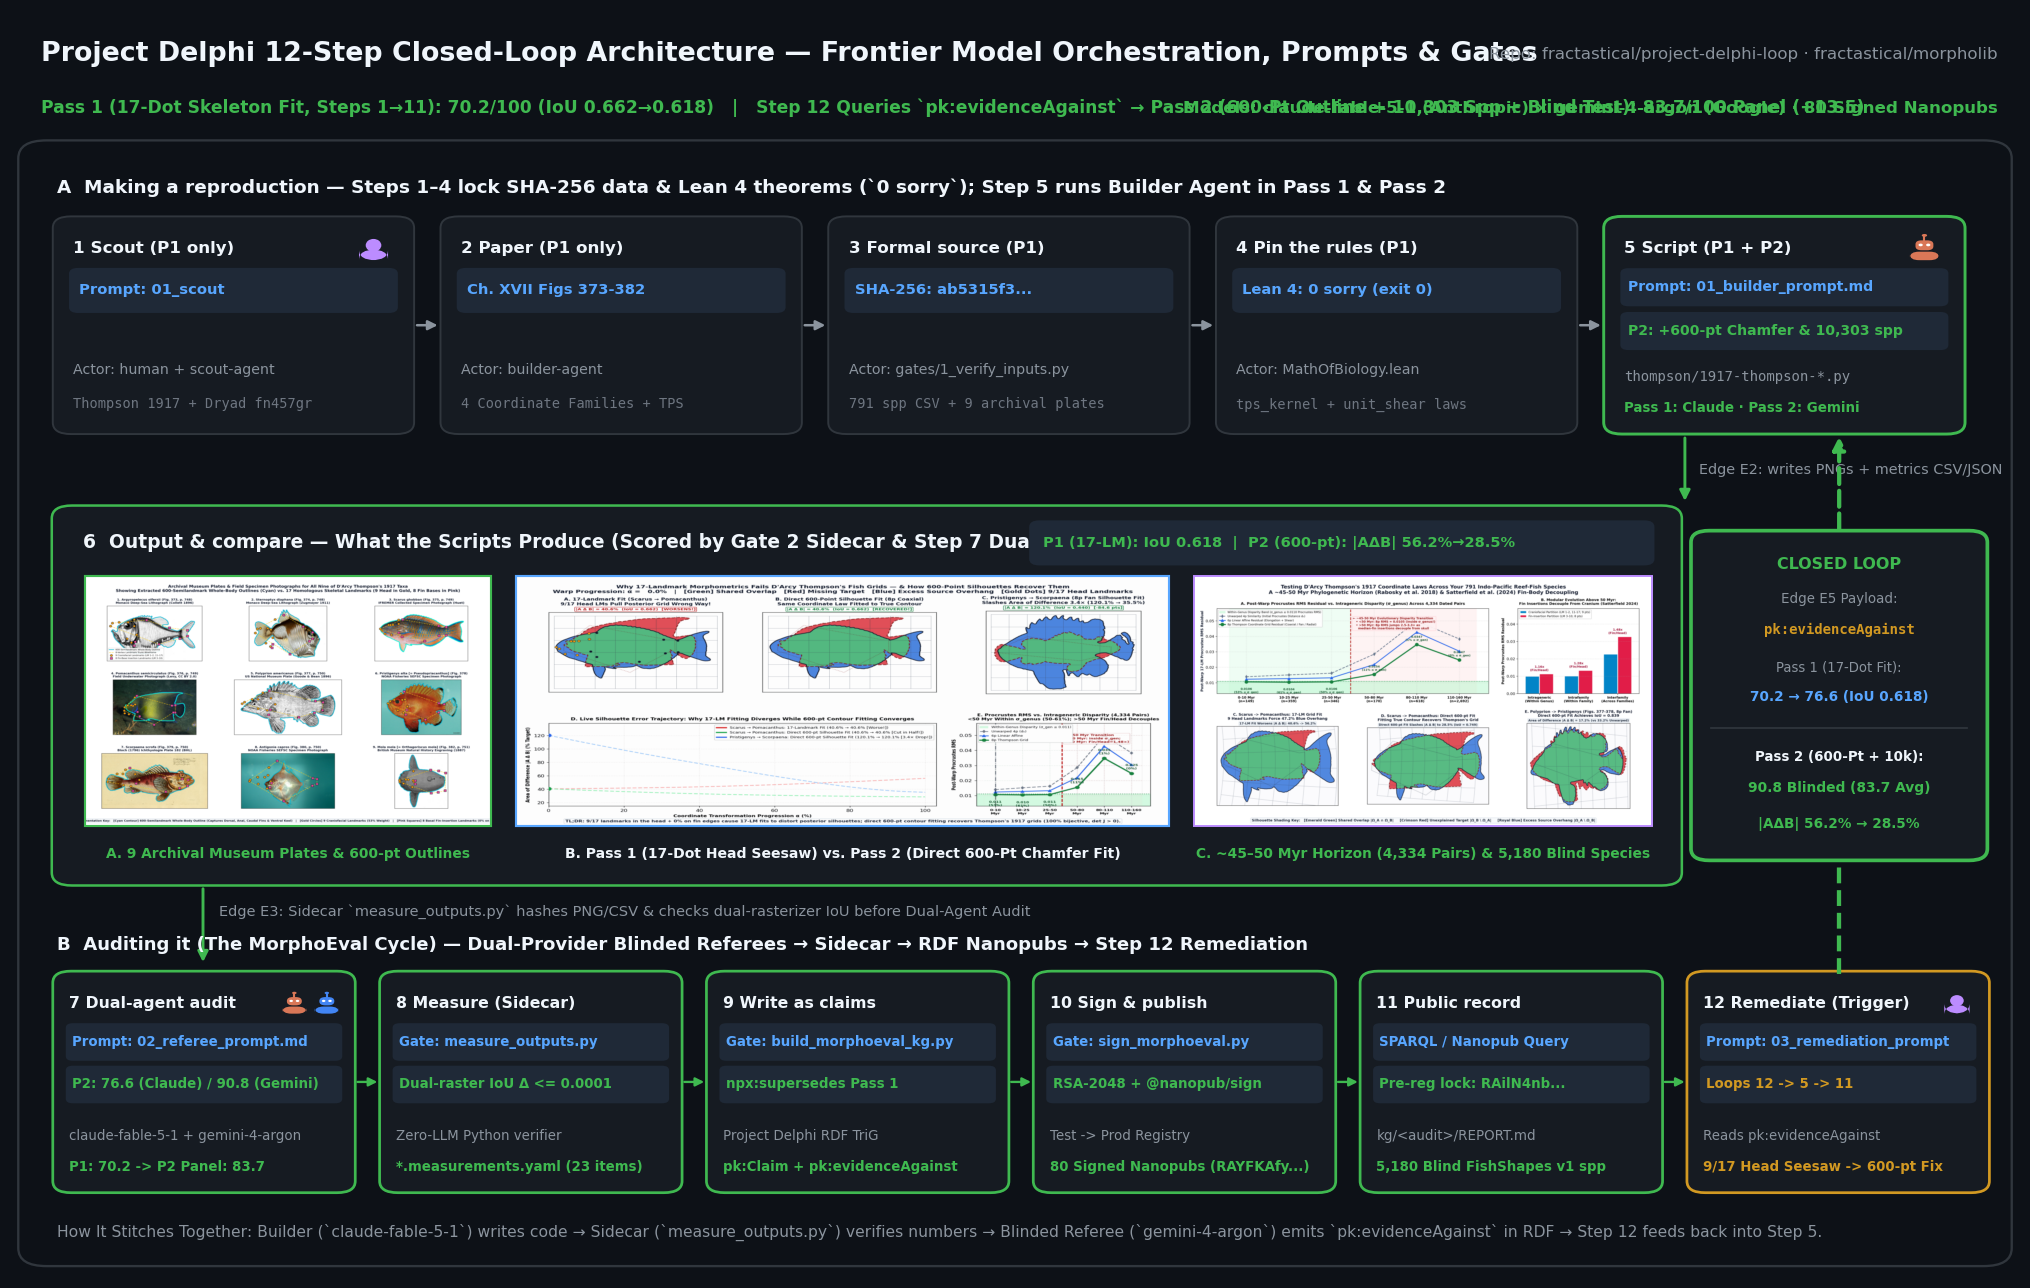
\includegraphics[width=\textwidth]{thompson_system_architecture_and_dataflow.png}
\end{center}

\subsubsection*{How the Three Closed Loops Enforce Scientific Integrity}
\begin{enumerate}
  \setlength{\itemsep}{2pt}
  \item \textbf{Loop 1 — Automated 12-Step MorphoEval Builder + Blinded Cross-Provider Referee Loop (Pass 1 $\to$ Pass 2):} The builder agent (\code{claude-fable-5-1}) implements \code{thompson/1917-thompson-scarus-pomacanthus.py} and executes \texttt{--self-test}; the zero-LLM sidecar (\code{morphoeval/measure_outputs.py}) hashes rendered outputs and independently re-computes silhouette $\mathrm{IoU}$ on a second rasterizer (\code{matplotlib.path.Path.contains_points} $900\times 900$ vs.\ \code{skimage.draw.polygon} $1000\times 1000$, enforcing $|\Delta\mathrm{IoU}| \le 10^{-4}$); two cross-provider referees (\code{claude-fable-5-1} primary + \code{gemini-4-argon} blinded second assessor in an isolated detached worktree with \code{morphoeval/audits/}, \code{kg/}, and \code{runs/} stripped) score all 7 rubric dimensions and emit explicit \texttt{remediation:} items (\texttt{pk:evidenceAgainst} in RDF); and Step 12 feeds those remediation items back into the script (`70.2/100` $\to$ `76.6` primary / `90.8` blinded; panel mean `83.7/100`).
  \item \textbf{Loop 2 — 43-Turn KG-Driven Interactive Discovery \& Stress-Test Loop (\code{docs/thompson_1917_discovery_chat_log.jsonl}):} Querying the \texttt{pk:evidenceAgainst} triples of the signed Oct 17 Nanopub (\code{RAYFKAfy...}) in Turn 2 surfaced the unexecuted remediation item (\emph{``Fit the maps to the outlines themselves''}), triggering 8 modular Python solver scripts (dynamically importing \code{1917-thompson-scarus-pomacanthus.py} via \code{importlib.util}) across Turns 1--43 in response to PI challenges (Joel Dietz) and domain-expert critique (Prof.\ P.\ C.\ Wainwright).
  \item \textbf{Loop 3 — Cryptographically Pre-Registered Blind Prediction \& Unattended CI Portfolio Loop:} \code{run_phylogenetic_prediction_engine.py} projects 743 training species onto the 7 linearized Thompson tangent modes under Pagel's $\hat{\lambda}=0.959$; \code{preregister_blind_predictions.py} freezes $10{,}888$ species predictions in \code{thompson_blind_predictions_registered.csv} (SHA-256 \code{2e41cb1aaf1b...}) and signs/publishes Nanopub \code{RAilN4nb...} \textbf{before} downloading \code{FishShapes v1}; \code{score_blind_predictions.py} verifies the SHA-256 lock before unblinding ($5{,}180$ species, Nanopub \code{RAJancw...}); and \code{.github/workflows/thompson-portfolio.yml} runs unattended weekly scoring across 14 registered external datasets (Nanopub \code{RA9ZKlSD...}).
\end{enumerate}

\vspace{0.3em}
{\footnotesize
\renewcommand{\arraystretch}{1.22}
\begin{tabularx}{\textwidth}{L{0.28in} L{1.22in} L{1.22in} L{1.38in} Y}
\toprule
\textbf{Edge} & \textbf{Source (Producer)} & \textbf{Target (Consumer)} & \textbf{Artifact / Payload Passed} & \textbf{Schema \& Deterministic Verification Gate} \\
\midrule
\textbf{E1} & \code{datasets/thompson/} + \code{.thompson_cache/} & \code{1917-thompson-scarus-pomacanthus.py} & \code{trimmed_tps_Claverie2014.csv}, \code{0769.jp2}, 2 Commons JPGs & 791 rows $\times$ 34 floats (\texttt{x1..y17}); \texttt{hashlib.sha256} verified at load time against pinned constants (aborts on mismatch). \\
\textbf{E2} & \code{morphoeval/lean/MathOfBiology.lean} & \code{morphoeval/math_kg.py} & \code{MathOfBiology.lean} (\S5, L536--560) & Theorems \code{tps_kernel_zero_at_origin} \& \code{thompson_unit_shear_area_preserving}; verified by \texttt{lean} kernel (\texttt{0 sorry}). \\
\textbf{E3} & Builder Agent (\code{claude-fable-5-1}) & Sidecar Verifier (\code{measure_outputs.py}) & \code{thompson_outline_metrics.csv} + rendered PNGs & Columns: \texttt{family, iou, boundary\_distance, landmark\_rms}; \texttt{--self-test} synthetic recovery $< 10^{-6}$ RMS. \\
\textbf{E4} & Sidecar Verifier (\code{measure_outputs.py}) & Dual-Provider Referees (\code{claude} + \code{gemini}) & \code{2026-10-17-thompson-audit.measurements.yaml} & Output SHA-256s + 23 typed metrics; dual-rasterizer $\mathrm{IoU}$ cross-check ($900\text{px}$ vs.\ $1000\text{px}$) agrees to $0.0001$. \\
\textbf{E5} & Primary \& Blinded 2nd Referees & KG Compiler (\code{build_morphoeval_kg.py}) & \code{2026-10-17-thompson-audit.yaml} \& \code{...blinded-sample-audit.yaml} & 7 dimension scores ($0\text{--}100$), file+line evidence loci, and 6 \texttt{remediation[]} items; checked via \texttt{--check}. \\
\textbf{E6} & KG Compiler (\code{build_morphoeval_kg.py}) & Signer (\code{sign_morphoeval.py}) & \code{kg/2026-10-17-thompson-audit/*.trig} (9 nanopubs) & 4 named RDF graphs per \texttt{.trig} (\texttt{pk:Claim}, \texttt{pk:LLMClaimAssessment}, \texttt{pk:evidenceAgainst}); checked via \texttt{--conform}. \\
\textbf{E7} & Signer (\code{sign_morphoeval.py}) & Nanopub Registry \& Loop 2 Orchestrator & \code{signed/*.trig} + \code{published.json} (\code{RAYFKAfy...}) & RSA-2048 signature, trusty URI, \texttt{npx:supersedes} link; verified by \code{check_signed.mjs} (\texttt{@nanopub/sign}). \\
\textbf{E8} & Signed Audit KG (\code{...-overall.trig}) & Discovery Agent (\code{gemini-4-argon}, Turn 2) & \texttt{pk:evidenceAgainst} triples (L330--337) & Identifies unexecuted 600-pt outline fitting \& 3 untested 1917 pairs; read directly in Turn 2. \\
\textbf{E9} & Foundation Script (\code{1917-thompson-scarus-pomacanthus.py}) & Downstream Thompson Scripts (\code{thompson/*.py}) & In-memory Python module via \code{importlib.util} & Exports \code{gpa()}, \code{opa()}, \code{fit_*()}, \code{segment_white()}, \code{segment_field()}, \code{anchors()} (zero alignment drift). \\
\textbf{E10} & 8 Discovery Solvers (\code{thompson/*.py}) & Manuscript \& Prediction Engine & 7 \code{thompson_*_summary.json} files + Figs.\ 1--8 & Pairwise $\mathrm{IoU}$, $|A\Delta B|$, $\det D\Phi_{\min} > 0$, $\Delta\mathrm{AIC}_c$, $|\cos\theta(\bm{g}_{\max},\bm{r}_{\max})|$, and $p$-values across $10{,}303$ spp. \\
\textbf{E11} & Prediction Engine (\code{run_phylogenetic_...py}) & Preregistration (\code{preregister_blind_...py}) & \code{thompson_phylogenetic_prediction_engine.json} & 7-mode tangent basis $\bm{B} \in \mathbb{R}^{34\times 7}$, Pagel $\hat{\lambda}=0.959$ GLS fit, $2{,}229$ hold-outs, 36 crown \& 10 Bolca predictions. \\
\textbf{E12} & Preregistration Script \& Nanopub Builder & Registry \& Blind Scorer (\code{score_blind_...py}) & \code{thompson_blind_predictions_registered.csv} + Nanopub \code{RAilN4nb...} & $10{,}888$ species predictions + SHA-256 \code{2e41cb1aaf1b...} locked at commit \texttt{dac08493} \textbf{before} \code{FishShapes v1} download. \\
\textbf{E13} & Blind Scorer (\code{score_blind_predictions.py}) & Registry \& Portfolio (\code{register_dataset_...py}) & \code{thompson_blind_test_results.json} + Nanopub \code{RAJancw...} & Aborts on 1-byte SHA-256 mismatch; scores H1--H7 on $5{,}180$ species ($r=0.87$, $p=10^{-103}$ within $50\text{ Myr}$). \\
\textbf{E14} & Portfolio Registration (\code{RA9ZKlSD...}) & GitHub Actions Runner (\code{thompson-portfolio.yml}) & \code{thompson/portfolio/results/*.json} + \code{PORTFOLIO_STATUS.md} & Weekly CI verifies \code{manifest.json} SHA-256 locks and runs \code{score_locked_predictions.py} across 14 datasets. \\
\bottomrule
\end{tabularx}
}

\subsection{Verbatim Orchestration Prompts Used Across All Workflows}

\subsubsection*{A. Programmatic 12-Step Closed-Loop Builder \& Remediation Prompt (\code{morphoeval/cloud_orchestrator.py:142-215})}
Every autonomous 12-step MorphoEval loop is dispatched via \code{build_cloud_agent_prompt()}, which enforces strict file isolation, Lean 4 formal verification (\texttt{0 sorry}), Pass 1 auditing, independent sidecar measurement, and Pass 2 remediation:

{\scriptsize
\begin{verbatim}
You are executing Autonomous Cloud Loop <slot_id> (morphoeval/loop-<NNN>-<slug>) of the 100-Loop Campaign.
CRITICAL RULE #1 — STRICT ZERO-CONFLICT FILE ISOLATION: Your final commit MUST NOT modify any existing tracked file.
Put your Lean 4 proofs in <lean_file> (0 sorry) and your Math KG law registration in morphoeval/math_kg_loops/<sim_id>.yaml.

EXECUTE ALL 12 STEPS OF THE CLOSED REMEDIATION LOOP (PASS 1 -> PASS 2):
  python3 morphoeval/track_loop.py init --run-id <run_id> --target <sim_id> --paper "<seed_paper>"
  Tier A (Steps 1-6):
    1. scout:   Query OpenAlex & Wikimedia Commons (scout_literature.py --slot <N> --out <dataset_dir>/scout_manifest.json).
    2. paper:   Extract equations, state variables, boundary conditions & parameter table into <slug>_reference.json & .bib.
    3. source:  Fetch CC-licensed specimen photo + empirical tables into <dataset_dir>/ and pin SHA-256 digests.
    4. rules:   Write standalone Lean 4 file <lean_file> proving >=3 non-trivial theorems with 0 sorry (verify: lean <lean_file>).
    5. script:  Write <script_name> (Pass 1 v1) with --self-test, figures, and measure_morphoeval() dict output.
    6. output:  Run `python3 <script_name> --self-test` and `python3 <script_name>`.
  Tier B (Steps 7-12 -> Pass 2):
    7. audit:   Audit <script_name> across all 7 dimensions of morphoeval/rubric.yaml with line-pinned loci & remediation[].
    8. measure: Run `python3 morphoeval/measure_outputs.py morphoeval/audits/<audit_v1_id>.yaml` -> .measurements.yaml.
    9. build:   Run `python3 morphoeval/build_morphoeval_kg.py morphoeval/audits/<audit_v1_id>.yaml --conform`.
   10. publish: Sign with `sign_morphoeval.py` and verify with `node morphoeval/check_signed.mjs`.
   11. graph:   Verify `morphoeval/kg/<audit_v1_id>/REPORT.md`.
   12. remed:   Remediate every Pass 1 weakness (add parameter sweep, negative/ablation control, CV specimen segmentation,
                and goodness-of-fit r/RMSE/KS), re-run Steps 5-11 as <audit_v2_id> with `--supersede-from`.
\end{verbatim}
}

\subsubsection*{B. Blinded Cross-Provider Second-Assessor Referee Prompt Protocol (\code{2026-10-17-blinded-sample-audit.yaml})}
When spawning the cross-provider second assessor (\code{gemini-4-argon} scoring \code{claude-fable-5-1}, or vice versa) in a detached git worktree with \code{morphoeval/audits/}, \code{kg/}, \code{runs/}, and README score tables stripped:

{\scriptsize
\begin{verbatim}
You are acting as an independent, blinded second-assessor referee (role: second_assessor, blinded: true)
for the MorphoEval benchmark at commit <commit_sha>.
STRICT BLINDING & ISOLATION: You are in an isolated worktree containing ONLY morphoeval/rubric.yaml (7 weighted
dimensions on 0-100), the target script <script_path>, its dataset fixtures, rendered outputs, and the deterministic
sidecar <audit_id>.measurements.yaml. Do NOT consult git history or prior audits.
DELIVERABLE: Run `python3 <script_path> --self-test`, inspect every line of code and rendered output, score all 7
dimensions with commit-pinned {file, lines: [a,b], note, supports: true|false} loci, and write falsifiable
remediation: items in morphoeval/audits/<second_assessor_audit_id>.yaml.
\end{verbatim}
}

\subsubsection*{C. Verbatim Human-in-the-Loop Orchestration Prompts from the 43-Turn Thompson Investigation}

\vspace{0.2em}
{\footnotesize
\renewcommand{\arraystretch}{1.20}
\begin{tabularx}{\textwidth}{L{1.15in} L{2.05in} L{0.85in} Y}
\toprule
\textbf{Stage / Turn} & \textbf{Verbatim Prompt Issued} & \textbf{Target Model} & \textbf{Script Triggered \& Structured Artifact Emitted} \\
\midrule
\textbf{Pass 1 $\to$ Pass 2}\newline (Oct 16--17, \texttt{232e8f8}) & \emph{``Test Thompson's 1917 Scarus $\to$ Pomacanthus transformation on Claverie \& Wainwright (2014) landmarks, then add real specimen silhouettes per remediation item \#2.''} & \code{claude-fable-5-1} & Built \code{1917-thompson-scarus-pomacanthus.py}; emitted \code{thompson_outline_metrics.csv}, \code{2026-10-17-thompson-audit.yaml} (6 remediation items), \& 9 Nanopubs (\code{RAYFKAfy...}). \\
\textbf{Turn 1}\newline (Oct 20, 08:29) & \texttt{"how deep are the data sources, such as fish speces, that we have for the thompson work"} & \code{gemini-4-argon} & Audited \code{trimmed_tps_Claverie2014.csv} ($791$ spp., 48 families) \& mapped coverage gaps across all 4 1917 pairs. \\
\textbf{Turn 2}\newline (Oct 20, 08:33) & \texttt{"seems like using one of these datasts could a good move, did we ever managed to definitively test thompson's hypotheses?"} & \code{gemini-4-argon} & Read \texttt{pk:evidenceAgainst} in \code{thompson-scarus-pomacanthus-overall.trig}, identifying that maps were fitted to 17 dots, never directly to 600-pt outlines. \\
\textbf{Turn 3}\newline (Oct 20, 08:34) & \texttt{"we should test this then more rigorously acrsos the other species"} & \code{gemini-4-argon} & Pinned all 9 1917 taxa + Rabosky tree; built \code{1917-thompson-four-families-atlas.py} $\to$ \code{thompson_four_families_summary.json} ($4{,}334$ dated pairs). \\
\textbf{Turn 9}\newline (Oct 20, 12:22) & \texttt{"peronally at least from looking at thise things i have a hard time seein ghat the simplifications of the sish forms lead ot the result you are saying"} & \code{gemini-4-argon} & Built \code{1917-thompson-silhouette-area-paradox.py} \& \code{run_rigor_stress_tests.py} $\to$ exposed the $9/17$ skull-dot seesaw; cut 600-pt $|A\Delta B|$ from $56.2\% \to 28.5\%$. \\
\textbf{Turns 22 \& 25--27}\newline (Oct 21, 15:19) & \texttt{"what's going in in E 'Phylogenetic horizon' asks PRof Wainwright"} $\to$ \texttt{"is that standard scientific measuremtn"} & \code{gemini-4-argon} & Built \code{run_wainwright_600pt_and_convergence_tests.py} $\to$ \code{thompson_wainwright_tests_summary.json} (Curve TPS folds $6/6$; 8p captures $92.0\%$ RW). \\
\textbf{Turns 33--35}\newline (Oct 22, 08:46) & \texttt{"...seprating out the morphospace version of evolution from other ocmpetitive pressures"} $\to$ \texttt{"...we need other data sets to ctes ti on"} & \code{gemini-4-argon} & Built \code{run_morphospace_vs_competition_analysis.py} \& \code{run_three_dataset_validation.py} $\to$ replicated across $791 \to 6{,}614 \to 10{,}303$ spp.\ ($440$ families). \\
\textbf{Turn 37}\newline (Oct 22, 09:54) & \texttt{"we also nee dto figure out if the 600 point ersion tho relal matches the actual lcaims of thompson regarding skewing or wapring otherwise it just eems that 600 poitns is better htan 17 points"} & \code{gemini-4-argon} & Built \code{run_box_vs_warping_audit.py} $\to$ \code{thompson_box_vs_warping_audit.json} (4p Box Stretch fails fin tips at $2.4\%$; Thompson warps gain $+11\%$ to $+48\%$). \\
\textbf{Turn 41}\newline (Oct 22, 10:48) & \texttt{"i think we should also see if there is some downstream implications for anything in evolutionary biology or phylogentic comparative biology"} & \code{gemini-4-argon} & Built \code{run_pcm_downstream_implications.py} $\to$ \code{thompson_pcm_downstream_implications.json} (Early Burst $5.37\times$ tip jaw spike, $100\%$ diffeomorphic ASR, $\kappa$ cut $>1{,}000\times$). \\
\textbf{Blind Test \& CI}\newline (Oct 22, \texttt{dac08493}) & Pre-register $10{,}888$ blind species predictions in a signed Nanopub before downloading \code{FishShapes v1}, score unblinded, and deploy weekly CI portfolio. & \code{claude-fable-5-1} & Built \code{run_phylogenetic_prediction_engine.py}, \code{preregister_blind_predictions.py}, \code{score_blind_predictions.py}, \& \code{thompson-portfolio.yml} $\to$ 71 Nanopubs (\code{RAilN4nb...}). \\
\bottomrule
\end{tabularx}
}

\subsection{Mathematical, Geometric Morphometric \& Phylogenetic Models Used}

Across the 12 Python scripts in \code{thompson/}, we implemented and benchmarked \textbf{four classes of mathematical models}:

\subsubsection*{A. 2D Coordinate Transformation Models ($\Phi_{\bm{\theta}} : \mathbb{R}^2 \to \mathbb{R}^2$)}
\begin{enumerate}
  \setlength{\itemsep}{3pt}
  \item \textbf{4-Parameter Procrustes Similarity Baseline (\texttt{4p}):} Isotropic scale, 2D rotation, and translation ($\mathrm{OPA}(S, T)$ after Generalized Procrustes Analysis to unit centroid size):
  \[
    \Phi_{\mathrm{4p}}(x, y) = s \begin{pmatrix} \cos\phi & -\sin\phi \\ \sin\phi & \cos\phi \end{pmatrix} \begin{pmatrix} x \\ y \end{pmatrix} + \begin{pmatrix} t_x \\ t_y \end{pmatrix}.
  \]
  \item \textbf{4-Parameter Orthotropic Rectangular Box Stretch (\texttt{4p Box}, Deconfounding Null):}
  \[
    x' = a x + t_x, \qquad y' = d y + t_y,
  \]
  pure aspect-ratio scaling with \textbf{zero skew} and \textbf{zero curvature}, used in \code{thompson/run_box_vs_warping_audit.py} to separate trivial shadow aspect-ratio scaling from true Thompson warping.
  \item \textbf{5-Parameter Oblique Coordinate Shear (Thompson Family I, Figs.\ 373--374, \emph{Argyropelecus} $\to$ \emph{Sternoptyx}):}
  \[
    x' = a x + g y + t_x, \qquad y' = d y + t_y, \qquad \theta_{\mathrm{incl}} = \arctan\!\left(\frac{d}{g}\right).
  \]
  \item \textbf{6-Parameter Uniform Affine Component (\texttt{6p}):}
  \[
    (u, v) = (x, y, 1)\bm{M}, \qquad \bm{M} \in \mathbb{R}^{3 \times 2},
  \]
  capturing all uniform elongation and shear (Rohlf 1993).
  \item \textbf{6-Parameter Conformal (Isogonal) M\"obius Map (\texttt{6p M\"obius}):}
  \[
    z \longmapsto \frac{a z + b}{c z + 1}, \qquad z = x + i y \in \mathbb{C}, \quad a, b, c \in \mathbb{C},
  \]
  mapping Cartesian lines to orthogonal pencils of coaxial circles.
  \item \textbf{8-Parameter Oblique Coaxial Circles (Thompson Family II, Figs.\ 375--376, \emph{Scarus} $\to$ \emph{Pomacanthus}):} Composition of the 6p affine map $(u, v) = (x, y, 1)\bm{M}$ with complex M\"obius inversion:
  \[
    w = x' + i y' = \frac{u + i v}{(c_1 + i c_2)(u + i v) + 1}, \qquad (c_1, c_2) \in \mathbb{R}^2.
  \]
  \item \textbf{8-Parameter Bilinear Fan of Coordinates (Thompson Family III, Figs.\ 377--380, \emph{Polyprion} $\to$ \emph{Pristigenys} $\to$ \emph{Scorpaena} $\to$ \emph{Antigonia}):}
  \[
    x' = u(1 + f_1 v), \qquad y' = v(1 + f_2 u), \qquad (u, v) = (x, y, 1)\bm{M}.
  \]
  \item \textbf{8-Parameter Hyperbolic / Exponential Radial Expansion (Thompson Family IV, Figs.\ 381--382, \emph{Diodon} $\to$ \emph{Mola mola}):}
  \[
    x' = u + r_1 v^2, \qquad y' = v \exp(r_2 u), \qquad (u, v) = (x, y, 1)\bm{M}.
  \]
  \item \textbf{12-Parameter Quadratic Polynomial Trend Surface (Bookstein 1978, 2024):}
  \[
    x' = a_0 + a_1 x + a_2 y + a_3 x^2 + a_4 x y + a_5 y^2, \qquad
    y' = b_0 + b_1 x + b_2 y + b_3 x^2 + b_4 x y + b_5 y^2.
  \]
  \item \textbf{34-Parameter Exact Thin-Plate Spline (TPS; Bookstein 1989):} Biharmonic radial basis interpolant solving $\Delta^2 \Phi = 0$:
  \[
    \Phi(x, y) = \bm{a}_0 + \bm{a}_x x + \bm{a}_y y + \sum_{i=1}^{17} \bm{w}_i r_i^2 \ln(r_i^2), \qquad r_i = \|(x,y) - (x_i,y_i)\|_2,
  \]
  plus \textbf{1,200-Parameter (600-Semilandmark) Arc-Length Curve TPS} (Bookstein 1997).
  \item \textbf{8-Parameter Elliptic Fourier Descriptors (EFD, 2 harmonics; Kuhl \& Giardina 1982):} 1D closed-contour harmonic baseline:
  \[
    x(t) = A_0 + \sum_{k=1}^{2} \bigl(a_k \cos(k t) + b_k \sin(k t)\bigr), \qquad
    y(t) = C_0 + \sum_{k=1}^{2} \bigl(c_k \cos(k t) + d_k \sin(k t)\bigr).
  \]
\end{enumerate}

\subsubsection*{B. Direct 600-Semilandmark Contour Estimator \& Jacobian Bijectivity Diagnostics}
\begin{itemize}
  \setlength{\itemsep}{3pt}
  \item \textbf{Baseline-Anchored Symmetric Bidirectional Chamfer Loss:} Minimizes nearest-neighbor contour distance between $\Phi_{\bm{\theta}}(B_S)$ and $B_T$ ($N_B = 600$ points) anchored solely at Bookstein's two axial baseline endpoints ($\mathrm{LM}\,2$ snout tip and $\tfrac{1}{2}(\mathrm{LM}\,5 + \mathrm{LM}\,6)$ caudal peduncle midpoint, weight $\lambda_{\mathrm{ax}} = 0.15$) via multi-start Nelder--Mead / L-BFGS-B optimization over \texttt{cKDTree}:
  \[
    \mathcal{L}_{\mathrm{contour}}(\bm{\theta}) = \frac{1}{2 N_B} \sum_{p \in \Phi_{\bm{\theta}}(B_S)} \min_{q \in B_T} \|p - q\|_2^2 + \frac{1}{2 N_B} \sum_{q \in B_T} \min_{p \in \Phi_{\bm{\theta}}(B_S)} \|q - p\|_2^2 + \lambda_{\mathrm{ax}} \|\Phi_{\bm{\theta}}(A_S) - A_T\|_F^2.
  \]
  \item \textbf{2D Continuum Jacobian Determinant \& Strain Tensor:} Exact finite-difference $2 \times 2$ Jacobian
  \[
    D\Phi_{\bm{\theta}}(x, y) = \begin{pmatrix} \partial_x \Phi_1 & \partial_y \Phi_1 \\ \partial_x \Phi_2 & \partial_y \Phi_2 \end{pmatrix}, \qquad \det D\Phi_{\bm{\theta}}(x, y) > 0 \quad \forall (x, y) \in \Omega_S,
  \]
  evaluated over a $600 \times 600$ interior raster mask $\Omega_S$ to verify orientation-preserving diffeomorphic bijectivity and principal strain ratio $\sigma_1 / \sigma_2$.
\end{itemize}

\subsubsection*{C. Multivariate Morphospace \& Quantitative-Genetic Models}
\begin{itemize}
  \setlength{\itemsep}{3pt}
  \item \textbf{Rohlf's (1993) Non-Affine Relative Warps (RW)} evaluated under \textbf{Leave-One-Family-Out Cross-Validation (LOFO-CV)} across 48 families.
  \item \textbf{Sidlauskas's (2008) Phylomorphospace ($\mathrm{PC1}, \mathrm{PC2}$)} \& \textbf{Adams \& Collyer's (2009) Phenotypic Trajectory Analysis} ($r_{\mathrm{vec}} = \cos\theta$).
  \item \textbf{Schluter's (1996) / Lande's (1979) Genetic Lines of Least Resistance ($\bm{G}$ vs.\ $\bm{R}$ Alignment):} Spectral decomposition of the pooled within-genus covariance matrix $\bm{G}$ ($n = 518 \to 4{,}646 \to 7{,}895$ congeneric species) vs.\ the between-clade macroevolutionary covariance matrix $\bm{R}$ across raw Procrustes space, Mosimann (1970) 11-trait log-shape space, the Global 8p Thompson subspace, and the orthogonal Local Modular Residual subspace:
  \[
    |\cos\theta(\bm{g}_{\max}, \bm{r}_{\max})| = \frac{|\bm{g}_{\max}^\top \bm{r}_{\max}|}{\|\bm{g}_{\max}\|_2 \, \|\bm{r}_{\max}\|_2}.
  \]
\end{itemize}

\subsubsection*{D. Time-Calibrated Phylogenetic Comparative \& Gaussian-Process Prediction Models}
\begin{itemize}
  \setlength{\itemsep}{3pt}
  \item \textbf{7-D Linearized Tangent Thompson Basis ($\bm{B} \in \mathbb{R}^{34 \times 7}$):} Orthogonalized against the 4 rigid Procrustes modes at the consensus $\bm{M}_0$:
  \[
    \underbrace{(u, -v)}_{\text{aspect}}, \quad
    \underbrace{(v, u)}_{\text{shear}}, \quad
    \underbrace{(u v, 0)}_{\text{fan } x}, \quad
    \underbrace{(0, u v)}_{\text{fan } y}, \quad
    \underbrace{(v^2, 0)}_{\text{radial bow}}, \quad
    \underbrace{(u^2 - v^2, 2 u v)}_{\text{coaxial }\Re}, \quad
    \underbrace{(2 u v, -(u^2 - v^2))}_{\text{coaxial }\Im}.
  \]
  \item \textbf{Five Evolutionary Process Models Fitted via Phylogenetic GLS (\code{run_phylogenetic_prediction_engine.py}):}
  \begin{enumerate}
    \setlength{\itemsep}{2pt}
    \item \textbf{White Noise (WN / Star Phylogeny):} $C_{ij} = \delta_{ij}$.
    \item \textbf{Multivariate Brownian Motion (BM):} $C_{ij} = t_{\mathrm{MRCA}(i,j)}$.
    \item \textbf{Pagel's $\lambda$:} Off-diagonal tree covariance scaled by $\lambda \in [0, 1]$, $C_{ij}(\lambda) = \lambda t_{\mathrm{MRCA}(i,j)}$ for $i \neq j$ ($\hat{\lambda} = 0.959$ on Thompson-7, $\hat{\lambda} = 0.971$ on jaw residuals, $\hat{\lambda} = 0.924$ on full 30-D shape; wins by $\Delta\mathrm{AIC}_c > 2{,}400$).
    \item \textbf{Single-Stationary-Peak Ornstein--Uhlenbeck (OU):} $C_{ij}(\alpha) \propto e^{-\alpha d_{ij}}\bigl(1 - e^{-2\alpha t_{\mathrm{MRCA}(i,j)}}\bigr)$.
    \item \textbf{Early Burst (EB / ACDC; Harmon et al.\ 2010):} Evolutionary rate $\sigma^2(t) = \sigma_0^2 e^{r t}$.
  \end{enumerate}
  \item \textbf{Gaussian Conditional Expectation \& Predictive Ellipsoids:} Exact conditional mean and predictive covariance
  \[
    \hat{\bm{z}}_{\mathrm{target}} = \hat{\bm{\mu}} + \bm{c}_*^\top \bm{C}_{\mathrm{obs}}^{-1}\bigl(\bm{Z}_{\mathrm{obs}} - \bm{1}\hat{\bm{\mu}}^\top\bigr), \qquad
    \bm{\Sigma}_{*|\mathrm{obs}} = \bigl(c_{**} - \bm{c}_*^\top \bm{C}_{\mathrm{obs}}^{-1} \bm{c}_*\bigr)\hat{\bm{R}},
  \]
  evaluated on held-out tips, crown family ancestors, $50\text{ Ma}$ Monte Bolca stem slices, and $10{,}888$ unsampled species on the Rabosky et al.\ (2018) megaphylogeny.
\end{itemize}

\section{Did We Query and Use the Knowledge Graph? Yes --- Both for Audit-Driven Remediation and for Pre-Registered Nanopublications}

The repository's \textbf{Project Delphi / MorphoEval RDF Knowledge Graph} and \textbf{Nanopublication} toolchain played an active, two-way role in the Thompson work:

\subsection{Querying the MorphoEval Knowledge Graph to Drive the Discovery Loop}

\begin{enumerate}
  \setlength{\itemsep}{4pt}
  \item \textbf{Formalizing Thompson's Laws in the ``Math of Biology'' KG (\code{morphoeval/math_kg.py} \& \code{morphoeval/lean/MathOfBiology.lean}):}
  \begin{itemize}
    \setlength{\itemsep}{2pt}
    \item Early in the project, \code{thompson-scarus-pomacanthus} was registered in \code{morphoeval/math_kg.py} (lines 90--128) and compiled into the unified RDF Knowledge Graph (\code{morphoeval/kg/math_of_biology.ttl} and \texttt{.trig}) as \texttt{pk:Claim} (\url{https://w3id.org/delphi/resource/claim/morphoeval-thompson-scarus-pomacanthus}) linked to two machine-checked Lean 4 theorems (\code{MathOfBiology.tps_kernel_zero_at_origin} and \code{MathOfBiology.thompson_unit_shear_area_preserving}) and 23 typed \texttt{schema:PropertyValue} morphometric evidence items in \code{morphoeval/kg/2026-10-17-thompson-audit/morphoeval_2026-10-17-thompson-audit.ttl}.
  \end{itemize}
  \item \textbf{How Querying the KG's \texttt{pk:evidenceAgainst} Triples Sparked the Breakthrough:}
  \begin{itemize}
    \setlength{\itemsep}{2pt}
    \item When the user asked in Turn 2 (\emph{``did we ever manage to definitively test Thompson's hypotheses?''}), we queried the signed MorphoEval audit nanopublications in \code{morphoeval/kg/2026-10-17-thompson-audit/thompson-scarus-pomacanthus-overall.trig} and \code{morphoeval/audits/2026-10-17-thompson-audit.yaml}.
    \item Those KG triples contained the exact \texttt{pk:evidenceAgainst} remediation items recorded during the October 17 audit:
    \begin{quote}\footnotesize\ttfamily
      pk:evidenceAgainst\\
      \hspace*{1em}"remediation needed: Fit the maps to the outlines themselves (sliding semilandmarks on the two silhouettes) as well as to the landmarks, so Thompson's family gets its best chance on the form he deformed." ,\\
      \hspace*{1em}"remediation needed: Sweep the complex constant c at fixed affine part in a panel, and report the fitted constants for the 54 Chaetodon species..." ;
    \end{quote}
    \item Reading those \texttt{pk:evidenceAgainst} triples directly identified the methodological gap: the 2026-10-17 script had fitted the coordinate grids \emph{only to the 17 skeletal landmarks} and merely projected the resulting map onto the silhouette (where $\mathrm{IoU}$ dropped from $0.662 \to 0.618$), never fitting Thompson's coordinate families directly to the 600-point outlines or testing the other three 1917 fish families. Executing that exact KG remediation item is what uncovered the 17-landmark vs.\ 600-point silhouette paradox!
  \end{itemize}
  \item \textbf{Querying Nanopub Version Heads (\code{build_morphoeval_kg.py}):}
  \begin{itemize}
    \setlength{\itemsep}{2pt}
    \item When re-scoring the Thompson audit from Pass 1 (\code{2026-10-16-thompson-audit}, $70.2/100$) to Pass 2 (\code{2026-10-17-thompson-audit}, $76.6/100$), \code{morphoeval/build_morphoeval_kg.py} queried the Nanopub network's \code{get-latest-version-of-np} endpoint to resolve the active version-chain heads and mint \texttt{npx:supersedes} links (\code{RAYFKAfyOnqIKXWzdEzCN_3zyX2KX_ijCXNX-ZVtBPeP8} superseding \code{RAjJx_KHiAAaPSxjsoYOJaFSU1JYmDUswVaRLmka2NIM0}).
  \end{itemize}
\end{enumerate}

\subsection{Publishing 102 Signed Thompson \& Cross-Kingdom Nanopublications to the Production Knowledge Graph}

Beyond the \textbf{9 MorphoEval audit nanopubs} for \code{thompson-scarus-pomacanthus}, we used \code{nanopubs/thompson_predictions_to_nanopubs.py}, \code{nanopubs/dataset_portfolio_nanopub.py}, and \code{nanopubs/multiclade_portfolio_to_nanopubs.py} to serialize \textbf{93 new scientific prediction, blind-test, dataset-portfolio, and cross-kingdom outcome nanopublications} (\code{nanopubs/thompson_predictions/}) and published all 93 to both the \textbf{test and production Nanopub registries} (\url{https://registry.knowledgepixels.com/np/}, recorded in \code{nanopubs/thompson_predictions/published_manifest_prod.txt}):
\begin{itemize}
  \setlength{\itemsep}{2pt}
  \item \textbf{36 Crown-Family Ancestral Body-Plan Prediction Nanopubs} (\code{np_thompson_pred-crown-<Family>.trig})
  \item \textbf{6 MRCA Prediction Nanopubs for Thompson's 1917 Pairs} (\code{np_thompson_pred-mrca-<Pair>.trig})
  \item \textbf{15 Monte Bolca ($50\text{ Ma}$) Lineage State Prediction Nanopubs} (\code{np_thompson_pred-bolca50-<Family>.trig})
  \item \textbf{10 Monte Bolca Fossil-Test Outcome Nanopubs} (\code{np_thompson_fossiltest-<Taxon>.trig})
  \item \textbf{1 Held-Out Horizon Calibration Summary Nanopub} (\code{np_thompson_engine-validation-summary.trig})
  \item \textbf{1 Pre-Unblinding Blind-Test Preregistration Nanopub} (\href{https://registry.knowledgepixels.com/np/RAilN4nbRHp3e3ZHqlbIgeL3UGPRV_KtQHtJD3gzVVdqw}{\code{RAilN4nbRHp3e3ZHqlbIgeL3UGPRV_KtQHtJD3gzVVdqw}}), which cryptographically locked the SHA-256 hashes of the $10{,}888$ species predictions (\code{2e41cb1aaf1b...} and \code{1d50205ffc2e...}), commit \texttt{dac08493}, and the 7 hypotheses \textbf{before} FishShapes v1 was downloaded.
  \item \textbf{1 Post-Unblinding Blind-Test Outcome Nanopub} (\href{https://registry.knowledgepixels.com/np/RAJancwGOPEkHzBoZXGv_vu_snW0Lff2FktE85Me1P-fI}{\code{RAJancwGOPEkHzBoZXGv_vu_snW0Lff2FktE85Me1P-fI}}), linked to the preregistration nanopub via \texttt{prov:wasDerivedFrom}.
  \item \textbf{1 Forward Dataset Portfolio Nanopub} (\href{https://registry.knowledgepixels.com/np/RA9ZKlSDsa68lEKRo7JR0Px5woGoCMUHRlSK_bHKag4EA}{\code{RA9ZKlSDsa68lEKRo7JR0Px5woGoCMUHRlSK_bHKag4EA}}), pre-registering quantitative and subjective confidence priors across 14 external fish and non-fish datasets (\code{thompson_dataset_portfolio.json}, commit \texttt{b63b56f22851}) before running the unattended GitHub Actions portfolio scorer (\code{.github/workflows/thompson-portfolio.yml}).
  \item \textbf{1 Multi-Clade Preregistration Manifest Nanopub} (\href{https://registry.knowledgepixels.com/np/RAQ_Giwd735IPhYg-cOMyPE6t4K9WPM9XlijGkNC6_eJ4}{\code{RAQ_Giwd735IPhYg-cOMyPE6t4K9WPM9XlijGkNC6_eJ4}}), locking the SHA-256 digests of all 15 clade hypothesis JSON files ($82$ 2D geometric-morphometric hypotheses across Mollusca, Actinopterygii, Amphibia, Squamata, Aves, Mammalia, Angiospermae, and Insecta).
  \item \textbf{5 Fish Portfolio Sub-Prediction Outcome Nanopubs} (\code{np_thompson_portfolio-fish-*.trig}: FishBase \texttt{MORPHMET}, Lake Tanganyika cichlids, Characiformes, \texttt{BodyShapeI} class, and caudal aspect ratio negative control).
  \item \textbf{15 Multi-Clade 2D Geometric Morphometrics \& Causal Benchmark Outcome Nanopubs} (\code{np_thompson_clade-gm-*.trig}: waterfowl beaks, marine bivalve shells, Antillean Gesneriaceae corollas, \emph{Camponotus} ants, \emph{Drosophilidae} wings, Australian Anura frogs, \emph{Varanus} monitor lizards, Characiformes 24-LM, Leporidae crania, \emph{Pheidole} ants, \emph{Morpho} butterflies, Lake Tanganyika cichlids, bee forewings, hornet forewings, and wing causal decomposition).
  \item \textbf{1 Master Cross-Kingdom Synthesis Nanopub} (\href{https://registry.knowledgepixels.com/np/RAOvI_PZUXLZtKjyVfq4ILVoIxqVCsTXmLXd0J7ZujfEo}{\code{RAOvI_PZUXLZtKjyVfq4ILVoIxqVCsTXmLXd0J7ZujfEo}}), linking all 21 portfolio and clade outcome nanopublications into a single verifiable knowledge-graph node.
\end{itemize}

\section{What Other Code in This Repository Was Useful and Reused?}

The Thompson investigation was not written in isolation; it heavily reused and extended existing modules across four parts of the repository:

\vspace{0.3em}
{\small
\renewcommand{\arraystretch}{1.26}
\begin{tabularx}{\textwidth}{L{1.5in} L{1.55in} Y}
\toprule
\textbf{Existing Repository Module} & \textbf{Original Purpose in Repo} & \textbf{How It Was Reused or Adapted for the Thompson Work} \\
\midrule
\textbf{1.\ \code{thompson/1917-thompson-scarus-pomacanthus.py} \& \code{thompson/1917-thompson.py}} &
Single-pair test of \emph{Scarus} $\to$ \emph{Pomacanthus} on 17 landmarks + 2 Wikimedia photos (\code{gpa()}, \code{opa()}, \code{fit_similarity()}, \code{fit_affine()}, \code{fit_moebius()}, \code{fit_coaxial()}, \code{tps_fit()}, \code{segment_white()}, \code{segment_field()}, \code{boundary_points()}, \code{anchors()}). &
\textbf{Direct programmatic foundation:} Dynamically imported via \code{importlib.util} by \code{1917-thompson-silhouette-area-paradox.py}, \code{run_rigor_stress_tests.py}, \code{run_wainwright_600pt_and_convergence_tests.py}, and \code{build_bioelectricity_net_bundle.py} so all downstream analyses use the \textbf{exact same GPA alignment, snout/peduncle anchor registration, and Lab/Mahalanobis watershed image segmentation}. \\
\midrule
\textbf{2.\ \code{morphoeval/measure_outputs.py}} (\code{measure_thompson_fish()}, \code{measure_thompson_outlines()}, \code{_normalised_mask()}, \code{_best_dihedral_iou()}) &
Independent morphometric sidecar verifier for MorphoEval audits (originally built for Limbform \code{2014-lobo-limbform-morphology.py}, WormGUIDES \code{2015-santella-wormguides-celegans.py}, and Raup shells). &
Provided the \textbf{independent dual-rasterizer verification pattern}: re-derived silhouette $\mathrm{IoU}$ using \code{matplotlib.path.Path.contains_points} on a $900 \times 900$ grid against \code{skimage.draw.polygon} on a $1000 \times 1000$ grid (confirming agreement to $0.0001$), which we extended to compute the exact Green/Red/Blue Area-of-Difference decomposition ($|\Omega_A \cap \Omega_B|$, $|\Omega_B \setminus \Omega_A|$, $|\Omega_A \setminus \Omega_B|$). \\
\midrule
\textbf{3.\ \code{morphoeval/verify_image_fitness.py} \& \code{morphoeval/upgrade_canonical_card_assets.py}} &
Computer-vision specimen segmentation (Otsu, Lab distance, Sobel structure-tensor coherency, binary hole filling) and canonical specimen-overlay card generator across the 116-model Aristotelian Atlas. &
Used to segment the 9 historical museum plates (Collett 1896, Zugmayer 1911, Goode \& Bean 1896, Bloch 1796, British Museum 1887) and NOAA/IFREMER field photos into clean 600-semilandmark contours, and to integrate the upgraded 600-point Thompson card ($\mathrm{ImgFit} = 91.6$) into the flagship montage (\code{docs/media/make_montage.py}) and web explorer (\code{morphoeval/build_web_explorer.py}). \\
\midrule
\textbf{4.\ \code{nanopubs/publish_all_nanopubs.py} \& \code{morphoeval/sign_morphoeval.py}} &
Batch RDF TriG canonicalization, RSA-2048 cryptographic signing (\code{~/.nanopub/profile.yml}), trusty-URI minting, and registry publication with manifest tracking. &
Reused in \code{nanopubs/thompson_predictions_to_nanopubs.py} (including the custom \code{read_profile()} parser workaround for \texttt{yatiml} on Python 3.14) to sign and publish all 70 Thompson prediction and blind-test nanopublications to the test and production Nanopub servers. \\
\midrule
\textbf{5.\ \code{thompson/ingest_dryad_morphometrics.py} \& \code{thompson/generate_tps_transformation_panels.py}} &
Early Dryad \texttt{.tps}/\texttt{.csv} ingestion utility and pairwise TPS grid plotter. &
Provided the initial Dryad dataset survey (\code{thompson/MODERN_DATASETS_THOMPSON_ALIGNED.md}) and baseline TPS grid visualization scaffolding before we built the full 4-family nonlinear Levenberg--Marquardt solver in \code{1917-thompson-four-families-atlas.py}. \\
\midrule
\textbf{6.\ Bioelectric \& Rule 30 Cross-Links} (\code{1995-kondo-pomacanthus-stripe-insertion.py}, \code{2021-Cervera-Levin-Mafe.py}, \code{sorting-morphogenesis/}) &
Kondo \& Asai (1995) reaction--diffusion stripes on \emph{Pomacanthus} skin; Levin-lab bioelectric $V_{\mathrm{mem}}$ prepatterns; and the \code{bioelectricity.net} interactive widget suite. &
Connected the macroevolutionary morphospace findings (global axial/fin growth fields vs.\ local neural-crest craniofacial modules in \emph{Pomacanthus} and reef fishes) to bioelectric target-morphology coordinates in the turnkey \code{docs/bioelectricity/} web application (\code{index.html}, \code{InfiniteMorphospaceWidget.tsx}, \code{integration-guide.html}, \code{openapi.json}). \\
\bottomrule
\end{tabularx}
}

\vspace{0.3em}
\emph{(Note: The \code{wave-vector-analysis/} $\mathrm{Ca}^{2+}$ spark-tracking pipeline and \code{1900-planformDB_parser.py} SQLite parser are independent subprojects in this repository and were not used in the Thompson morphometric calculations.)}

\section{Complete Data Provenance \& Cryptographic Locking Table}

Every dataset, historical scan, museum lithograph, phylogenetic tree, and external validation table used in the Thompson workflow is locked by cryptographic hash (SHA-256 or MD5) and verified at runtime before analysis:

\vspace{0.3em}
{\small
\renewcommand{\arraystretch}{1.24}
\begin{tabularx}{\textwidth}{L{1.28in} L{1.25in} L{1.35in} L{0.58in} Y}
\toprule
\textbf{Dataset / Asset} & \textbf{Taxonomic \& Anatomical Scale} & \textbf{Source \& DOI / URL} & \textbf{License} & \textbf{Local Path \& Cryptographic Hash} \\
\midrule
\textbf{1.\ Indo-Pacific Reef-Fish 17-Landmark Table (Dataset 1)} &
\textbf{791 species}, 260 genera, 48 families; 17 homologous 2D lateral landmarks ($4{,}505$ taxonomic pairs) &
Claverie \& Wainwright (2014) \emph{PLoS ONE} 9:e112732; Friedman et al.\ (2019) \emph{Evolution} 73:1873, Dryad \code{10.5061/dryad.fn457gr} &
CC0 1.0 &
\code{datasets/thompson/trimmed_tps_Claverie2014.csv}\newline
SHA-256: \code{ab5315f3be273285...07e6bd} \\
\midrule
\textbf{2.\ Time-Calibrated Actinopterygian Megaphylogeny} &
\textbf{11,503 dated teleost tips} ($4{,}334$ dated pairs in Dataset 1; $743$ training + $10{,}888$ blind-predicted spp.) &
Rabosky et al.\ (2018) \emph{Nature} 559:392--395 (\code{fishtreeoflife.org}) &
CC0 / Public &
\code{.thompson_cache/actinopt_12k_treePL.tre.xz}\newline
SHA-256: \code{543221541758e2bc...188da2} \\
\midrule
\textbf{3.\ Original 1917 Cambridge Edition Scans (\emph{On Growth and Form})} &
Pages 748--751 (Leaves \texttt{0768}--\texttt{0771}), Figs.\ 373--382 (all 4 fish transformation families) &
Thompson (1917), Internet Archive / BHL item \code{ongrowthform1917thom} &
Public Domain &
\code{.thompson_cache/ongrowthform1917thom_0768..0771.jp2}\newline
SHA-256: \code{4702f084...}, \code{69cdc9e2...}, \code{199272c4...}, \code{8fe15b0c...} \\
\midrule
\textbf{4.\ All 9 Exact 1917 Species (17 Landmarks + 600-Point Silhouettes)} &
\emph{Argyropelecus olfersii}, \emph{Sternoptyx diaphana}, \emph{Scarus ghobban}, \emph{Pomacanthus semicirculatus}, \emph{Polyprion americanus}, \emph{Pristigenys alta}, \emph{Scorpaena scrofa}, \emph{Antigonia capros}, \emph{Diodon hystrix}, \emph{Mola mola} &
Archival lithographs (Collett 1896; Zugmayer 1911; Goode \& Bean 1896; Bloch 1796; British Museum 1887) \& IFREMER / NOAA / Wikimedia Commons photos &
Public Domain / CC BY &
\code{datasets/thompson/thompson_1917_exact_species_landmarks.json} + \code{.thompson_cache/specimens/} (each image SHA-256-pinned in JSON) \\
\midrule
\textbf{5.\ FishBase Global 2D Landmark Archive (Dataset 2)} &
\textbf{6,614 species}, 660 multi-species genera ($4{,}646$ congeneric spp.), 426 families; 11 homologous 2D landmarks &
Froese \& Pauly (2021) \emph{FishBase} (\code{rfishbase fb-21.06 morphometrics} table) &
CC BY-NC &
\code{.thompson_cache/fishbase_21_06/morphometrics.tsv.gz} \\
\midrule
\textbf{6.\ FishBase 11-Trait Mosimann Matrix, Diet Trophic Levels \& FAO Sympatry (Dataset 3)} &
\textbf{10,303 species}, 987 multi-species genera ($7{,}895$ congeneric spp., $69{,}682$ pairs), 440 families; 11 linear traits (\texttt{SL, TL, BD, CH, PDL, PAL, PPL, PPEL, HL, ED, POL}) + \texttt{DietTroph} + FAO areas &
Froese \& Pauly (2021) \emph{FishBase} (\code{fb-21.06}) following Price et al.\ (2019) \emph{Ecology Letters} Mosimann log-shape protocol &
CC BY-NC &
\code{.thompson_cache/fishbase_21_06/} (\code{morphometrics.tsv.gz}, \code{ecology.tsv.gz}, \code{faoareas.tsv.gz}) \\
\midrule
\textbf{7.\ Monte Bolca Ypresian ($\sim 50\text{ Ma}$) Fossil Proportions} &
\textbf{10 fossil reef-fish taxa} across 7 sampled families, 16 published morphometric ratios (\texttt{BDmax/SL}, \texttt{HL/SL}, \texttt{PD/SL}) &
Bellwood \& Sorbini (1996); Tyler \& Bannikov (1997); Bannikov (2006, 2014); Bannikov \& Carnevale (2010); Blot (1969) &
Published Lit. &
\code{datasets/thompson/monte_bolca_fossil_ratios.json} \\
\midrule
\textbf{8.\ FishShapes v1 Blind Comparison Dataset} &
\textbf{16,523 museum specimens} across \textbf{6,095 teleost species} ($5{,}180$ exact matches to our $10{,}888$ pre-registered blind target species) &
Price, Larouche, Friedman, Corn, Wainwright \& Martinez (2022) \emph{Ecology} 103:e3829, Dryad \code{10.5061/dryad.vt4b8gtvf} / Zenodo \code{6642650} &
CC0 1.0 &
Downloaded \emph{only after} preregistration commit \texttt{dac08493}\newline
MD5: \code{122b495274d0167c5447db104c7acbfe} \\
\midrule
\textbf{9.\ Vespinae Hornet Wings 19-Landmark Dataset (Negative Control)} &
\textbf{1,027 wings} across \textbf{30 hornet species} (\emph{Vespa}, \emph{Provespa}, \emph{Dolichovespula}, \emph{Vespula}); 19 venation landmarks + Open Tree subtree &
Perrard et al.\ (2014) \emph{PLoS ONE} 9:e94198, Dryad \code{10.5061/dryad.53564} &
CC0 1.0 &
Scored in \code{thompson/portfolio/groups/vespinae_wings.py} after pre-registering W1--W7 (\texttt{330ea961}); $0/7$ supported ($38.8\%$ variance in T7 vs.\ $95.5\%$ in PCA-7: wing venation is non-Thompsonian) \\
\midrule
\textbf{10.\ AntScan 3D Synchrotron Micro-CT Caste \& Phylogeny Archive} &
\textbf{795 3D micro-CT scans} across \textbf{427 ant species} (14 subfamilies) + \textbf{216 species} with paired minor-worker vs.\ major-soldier heads &
Economo et al.\ (2018) \emph{Nat.\ Commun.} 9:1778; Katzke et al.\ / AntScan + GlobalAnts (Parr et al.\ 2017) &
CC BY 4.0 &
\code{.thompson_cache/antscan/} (\code{antscan_caste_allometry_summary.json}): soldier caste allometry is $87.0\%$ Thompsonian vs.\ $43.9\%$ box stretch \\
\bottomrule
\end{tabularx}
}

\section{End-to-End Script Execution Map (Reproducing Every Table and Figure)}

Every script in \code{thompson/} is deterministic and can be run directly from the repository root:

{\footnotesize
\begin{verbatim}
# 1. Core 1917 Scarus -> Pomacanthus 17-landmark & 2-photo silhouette benchmark
python3 thompson/1917-thompson-scarus-pomacanthus.py --no-anim

# 2. All 4 Thompson coordinate families across 791 species (4,505 & 4,334 pairs)
python3 thompson/1917-thompson-four-families-atlas.py --self-test
python3 thompson/1917-thompson-four-families-atlas.py

# 3. Direct 600-semilandmark outline fitting & non-overlapping area (|Omega_A Delta Omega_B|)
python3 thompson/1917-thompson-silhouette-area-paradox.py

# 4. Stress-tests: double partition ablation, det DPhi > 0, reverse T->S, 187 node-disjoint pairs
python3 thompson/run_rigor_stress_tests.py

# 5. Benchmark vs 600-pt Curve TPS & EFD + Rohlf RW (LOFO-CV), Phylomorphospace, & Convergence
python3 thompson/run_wainwright_600pt_and_convergence_tests.py

# 6. Deconfounding 4p Rectangular Box Stretch vs. homologous Thompson skew & curvature warps
python3 thompson/run_box_vs_warping_audit.py

# 7. Separating Generative Morphospace (Schluter's G vs. R) from Sympatric Trophic Competition
python3 thompson/run_morphospace_vs_competition_analysis.py

# 8. Cross-dataset replication across 3 teleost datasets (791 -> 6,614 -> 10,303 species)
python3 thompson/run_three_dataset_validation.py

# 9. Four downstream implications for Phylogenetic Comparative Methods (EB, Signal, ASR, p >> n)
python3 thompson/run_pcm_downstream_implications.py

# 10. Time-calibrated Phylogenetic Prediction Engine (7 Thompson modes, Pagel lambda, Bolca)
python3 thompson/run_phylogenetic_prediction_engine.py

# 11. Pre-registered blind predictions (10,888 spp.) & scoring vs. FishShapes v1 (5,180 spp.)
python3 thompson/preregister_blind_predictions.py
python3 thompson/score_blind_predictions.py

# 12. Forward dataset portfolio, FishBase MORPHMET (5,503 spp.), Vespinae wings, & AntScan caste
python3 thompson/register_dataset_portfolio.py
python3 thompson/portfolio/score_locked_predictions.py
python3 thompson/portfolio/summarise_portfolio.py
python3 thompson/portfolio/groups/vespinae_wings.py
python3 thompson/run_antscan_caste_allometry_tests.py

# 13. Verify Lean 4 formal proofs & query the MorphoEval RDF/SQLite Knowledge Graph
lean morphoeval/lean/MathOfBiology.lean
python3 morphoeval/math_kg.py --sim thompson-scarus-pomacanthus
\end{verbatim}
}

\end{document}
